\documentclass[]{article}

% Imported Packages
%------------------------------------------------------------------------------
\usepackage{amssymb}
\usepackage{amstext}
\usepackage{amsthm}
\usepackage{amsmath}
\usepackage{enumerate}
\usepackage{fancyhdr}
\usepackage[margin=1in]{geometry}
\usepackage{graphicx}
%\usepackage{extarrows}
%\usepackage{setspace}
%------------------------------------------------------------------------------

% Header and Footer
%------------------------------------------------------------------------------
\pagestyle{plain}  
\renewcommand\headrulewidth{0.4pt}                                      
\renewcommand\footrulewidth{0.4pt}                                    
%------------------------------------------------------------------------------

% Title Details
%------------------------------------------------------------------------------
\title{Deliverable \#2 Template}
\author{SE 3A04: Software Design II -- Large System Design}
\date{}                               
%------------------------------------------------------------------------------

% Document
%------------------------------------------------------------------------------
\begin{document}

\maketitle	
\noindent{\bf Tutorial Number:} T03\\
{\bf Group Number:} G07 \\
{\bf Group Members:} 
\begin{itemize}
	\item Farid Bastoros 
	\item Neha Bhatla
	\item Omar Alam
	\item Luka Mahrt-Smith
	\item Aidan Lao
\end{itemize}

\section*{IMPORTANT NOTES}
\begin{itemize}
	%	\item You do \underline{NOT} need to provide a text explanation of each diagram; the diagram should speak for itself
	\item Please document any non-standard notations that you may have used
	\begin{itemize}
		\item \emph{Rule of Thumb}: if you feel there is any doubt surrounding the meaning of your notations, document them
	\end{itemize}
	\item Some diagrams may be difficult to fit into one page
	\begin{itemize}
		\item Ensure that the text is readable when printed, or when viewed at 100\% on a regular laptop-sized screen.
		\item If you need to break a diagram onto multiple pages, please adopt a system of doing so and thoroughly explain how it can be reconnected from one page to the next; if you are unsure about this, please ask about it
	\end{itemize}
	\item Please submit the latest version of Deliverable 1 with Deliverable 2
	\begin{itemize}
		\item Indicate any changes you made.
	\end{itemize}
	\item If you do \underline{NOT} have a Division of Labour sheet, your deliverable will \underline{NOT} be marked
\end{itemize}

\newpage
\section{Introduction}
\label{sec:introduction}
% Begin Section

This section should provide an brief overview of the entire document.

\subsection{Purpose}
\label{sub:purpose}
% Begin SubSection
This document provides a high-level overview of the Shroomify system architecture, outlining the core design principles, subsystems, and the rationale behind architectural choices. It is intended for internal stakeholders involved in the development of Shroomify, including software engineers, project managers, investors, domain experts, and system architects. Prior technical knowledge is beneficial but not required for understanding this document. 
% End SubSection

\subsection{System Description}
\label{sub:system_description}
% Begin SubSection
Give a brief description of the system. This could be a paragraph or two to give some context to this document.

% End SubSection

\subsection{Overview}
\label{sub:overview}
% Begin SubSection
This is Deliverable 2 of the Shroomify project and provides a general description of the system architecture. It considers the requirements, use cases, and design decisions outlined in Deliverable 1. Section 2 has an Analysis Class Diagram that represents the major classes and how they relate to each other from our requirements analysis. This diagram establishes the foundation for the organization of the system internally and ensures that design is high in cohesion and low in coupling among its components. Section 3 presents a description of the Architectural Design of Shroomify. In this section, we define the chosen architectural pattern and discuss specific design decisions. Section 4 focused on Class Responsibility Collaboration (CRC) Cards. These cards capture the responsibilities and communications of each class within the system, detailing exactly how the individual components interact to satisfy the demands of the system.

% End SubSection

% End Section
\clearpage
\section{Analysis Class Diagram}
\label{sec:analysis_class_diagram}
% Begin Section
This section should provide an analysis class diagram for your application.
\begin{figure}[h]
    \centering
    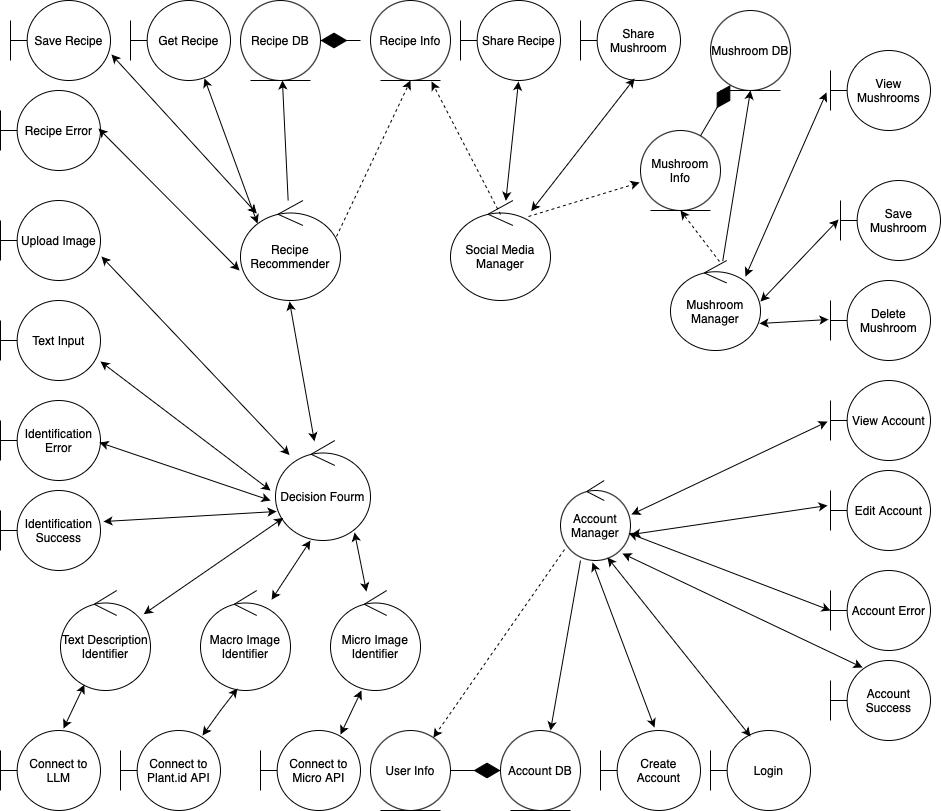
\includegraphics[width=1\textwidth]{AnalysisClassDiagram.png}
    \caption{Analysis Class Diagram}
    \label{fig:sample}
\end{figure}
% End Section

\clearpage
\section{Architectural Design}
\label{sec:architectural_design}
% Begin Section
This section should provide an overview of the overall architectural design of your application. Your overall architecture should show the division of the system into subsystems with high cohesion and low coupling.

\subsection{System Architecture}
\label{sub:system_architecture}
% Begin SubSection
\begin{itemize}
	\item Identify and explain the overall architecture of your system
	\item Be sure to clearly state the name of the architecture you used (this is the name of the architectural pattern, not the name of your system)
	\item Provide the reasoning and justification of the choice of architecture
	\item Provide a structural architecture diagram showing the relationship among the subsystems (if appropriate)
	\item List any design alternatives you considered, but eliminated (and explain why you eliminated them)
\end{itemize}
% End SubSection

\subsection{Subsystems}
\label{sub:subsystems}
% Begin SubSection
 Provide a list of your subsystems, with a brief description of each. Be sure to document its purpose and relationship to other subsystems.
 \subsubsection{Subsystem Overview}
Our system is divided into five main subsystems: \textbf{Decision Forum, Mushroom Management, Account Management, Social Media Management, and Recipe Recommendation}. These subsystems interact to provide users with a seamless experience in identifying mushrooms, managing their findings, and sharing information.

\subsubsection{Decision Forum}
The \textbf{Decision Forum} subsystem is responsible for identifying mushrooms. It contains the \textbf{machine learning algorithm} that classifies mushrooms based on user-provided descriptions and \textbf{computer vision technology} that analyzes images to determine species. If the identification confidence is low, users can also post images and descriptions to receive verification from the community.

\paragraph{Purpose}
Automates mushroom identification using AI and provides a space for community-based verification.

\paragraph{Relationship to Other Subsystems}
\begin{itemize}
    \item Works with \textbf{Mushroom Management} to store confirmed identifications.
    \item Interfaces with \textbf{Account Management} to associate identifications with users.
    \item Can interact with \textbf{Social Media Management} for users to share identification discussions.
\end{itemize}

\subsubsection{Mushroom Management}
The \textbf{Mushroom Management} subsystem serves as a \textbf{personal dictionary} of previously identified mushrooms. It allows users to view mushrooms they’ve found in the past, track their quantity, and access relevant information, including images and descriptions.

\paragraph{Purpose}
Stores and displays user-identified mushrooms but does \textbf{not} perform identification itself.

\paragraph{Relationship to Other Subsystems}
\begin{itemize}
    \item Retrieves identification results from \textbf{Decision Forum} and saves them.
    \item Integrates with \textbf{Account Management} to store mushroom data within user profiles.
    \item Interfaces with \textbf{Recipe Recommendation} to provide relevant recipes for identified mushrooms.
\end{itemize}

\subsubsection{Account Management}
The \textbf{Account Management} subsystem handles user authentication, profile settings, and data storage. It maintains a personalized record of identified mushrooms and user activity.

\paragraph{Purpose}
 % End SubSection

% End Section
\clearpage	
\section{Class Responsibility Collaboration (CRC) Cards}
\label{sec:class_responsibility_collaboration_crc_cards}
% Begin Section
This section should contain all of your CRC cards.

\begin{itemize}
	\item Provide a CRC Card for each identified class
	% \item Please use the format outlined in tutorial, i.e., 
	\begin{table}[ht]
		\centering
		\begin{tabular}{|p{6cm}|p{6cm}|}
		\hline 
		\multicolumn{2}{|l|}{\textbf{Class Name: Recipe Recommender (Controller)}} \\
		\hline
		\textbf{Responsibility:} & \textbf{Collaborators:} \\
		\hline
		Knows Get Recipe & Get Recipe\\
		Knows Save Recipe & Save Recipe\\
		Knows Recipe Error & Recipe Error\\
		Knows Recipe DB & Recipe DB\\
		Knows Decision Fourm & Decision Fourm\\
		Knows Recipe Info & Recipe Info\\
		\vspace{1in} & \\
		\hline
		\end{tabular}
	\end{table}
	\begin{table}[ht]
		\centering
		\begin{tabular}{|p{6cm}|p{6cm}|}
		\hline 
		\multicolumn{2}{|l|}{\textbf{Class Name: Recipe DB (Entity)}} \\
		\hline
		\textbf{Responsibility:} & \textbf{Collaborators:} \\
		\hline
		Knows Recipe Recommender & Recipe Recommender \\
		Knows Recipe Info & Recipe Info \\
		\vspace{1in} & \\
		\hline
		\end{tabular}
	\end{table}
	\begin{table}[ht]
		\centering
		\begin{tabular}{|p{6cm}|p{6cm}|}
		\hline 
		\multicolumn{2}{|l|}{\textbf{Class Name: Get Recipe (Boundary)}} \\
		\hline
		\textbf{Responsibility:} & \textbf{Collaborators:} \\
		\hline
		Knows Recipe Recommender & Recipe Recommender \\
		Handles click event of “Get Recipe” button & \\  
		\vspace{1in} & \\
		\hline
		\end{tabular}
	\end{table}
	\begin{table}[ht]
		\centering
		\begin{tabular}{|p{6cm}|p{6cm}|}
		\hline 
		\multicolumn{2}{|l|}{\textbf{Class Name: Save Recipe (Boundary)}} \\
		\hline
		\textbf{Responsibility:} & \textbf{Collaborators:} \\
		\hline
		Knows Recipe Recommender & Recipe Recommender \\
		Handles click event of “Save Recipe” button & \\
		\vspace{1in} & \\
		\hline
		\end{tabular}
	\end{table}
	\begin{table}[ht]
		\centering
		\begin{tabular}{|p{6cm}|p{6cm}|}
		\hline 
		\multicolumn{2}{|l|}{\textbf{Class Name: Recipe Error (Boundary)}} \\
		\hline
		\textbf{Responsibility:} & \textbf{Collaborators:} \\
		\hline
		Knows Recipe Recommender & Recipe Recommender \\
		Handles Get Recipe error events & \\
		Handles Save Recipe error events & \\
		\vspace{1in} & \\
		\hline
		\end{tabular}
	\end{table}
	\begin{table}[ht]
		\centering
		\begin{tabular}{|p{6cm}|p{6cm}|}
		\hline 
		\multicolumn{2}{|l|}{\textbf{Class Name: Decision Fourm (Controller)}} \\
		\hline
		\textbf{Responsibility:} & \textbf{Collaborators:} \\
		\hline
		Knows Upload Image & Upload Image \\
		Knows Text Input & Text Input \\
		Knows Identification Error & Identification Error \\
		Knows Identification Success & Identification Success \\
		Knows Text Description Identifier &  Text Description Identifier \\
		Knows Macro Image Identifier & Macro Image Identifier \\
		Knows Micro Image Identifier & Micro Image Identifier \\
		Knows Recipe Recommender & Recipe Recommender \\

		\vspace{1in} & \\
		\hline
		\end{tabular}
	\end{table}
	\begin{table}[ht]
		\centering
		\begin{tabular}{|p{6cm}|p{6cm}|}
		\hline 
		\multicolumn{2}{|l|}{\textbf{Class Name: Text Description Identifier (Controller)}} \\
		\hline
		\textbf{Responsibility:} & \textbf{Collaborators:} \\
		\hline
		Knows Connect to LLM & Connect to LLM \\
		Knows Decision Fourm & Decision Fourm \\ 
		\vspace{1in} & \\
		\hline
		\end{tabular}
	\end{table}
	\begin{table}[ht]
		\centering
		\begin{tabular}{|p{6cm}|p{6cm}|}
		\hline 
		\multicolumn{2}{|l|}{\textbf{Class Name: Macro Image Identifier (Controller)}} \\
		\hline
		\textbf{Responsibility:} & \textbf{Collaborators:} \\
		\hline
		Knows Connect to plant.id API & Connect to plant.id API \\
		Knows Decision Fourm & Decision Fourm \\ 
		\vspace{1in} & \\
		\hline
		\end{tabular}
	\end{table}
	\begin{table}[ht]
		\centering
		\begin{tabular}{|p{6cm}|p{6cm}|}
		\hline 
		\multicolumn{2}{|l|}{\textbf{Class Name: Micro Image Identifier (Controller)}} \\
		\hline
		\textbf{Responsibility:} & \textbf{Collaborators:} \\
		\hline
		Knows Connect to Micro API & Connect to Micro API \\
		Knows Decision Fourm & Decision Fourm \\ 
		\vspace{1in} & \\
		\hline
		\end{tabular}
	\end{table}
	\begin{table}[ht]
		\centering
		\begin{tabular}{|p{6cm}|p{6cm}|}
		\hline 
		\multicolumn{2}{|l|}{\textbf{Class Name: Upload Image (Boundary)}} \\
		\hline
		\textbf{Responsibility:} & \textbf{Collaborators:} \\
		\hline
		Knows Decision Fourm & Decision Fourm \\
		Handles click event of “Upload Image” button & \\
		\vspace{1in} & \\
		\hline
		\end{tabular}
	\end{table}
	\begin{table}[ht]
		\centering
		\begin{tabular}{|p{6cm}|p{6cm}|}
		\hline 
		\multicolumn{2}{|l|}{\textbf{Class Name: Text Input (Boundary)}} \\
		\hline
		\textbf{Responsibility:} & \textbf{Collaborators:} \\
		\hline
		Knows Decision Fourm & Decision Fourm \\
		Handles click event of “Text Input” button & \\
		\vspace{1in} & \\
		\hline
		\end{tabular}
	\end{table}
	\begin{table}[ht]
		\centering
		\begin{tabular}{|p{6cm}|p{6cm}|}
		\hline 
		\multicolumn{2}{|l|}{\textbf{Class Name: Identification Error (Boundary)}} \\
		\hline
		\textbf{Responsibility:} & \textbf{Collaborators:} \\
		\hline
		Knows Decision Fourm & Decision Fourm \\
		Handles Upload Image error events & \\
		Handles Text Input error events & \\
		\vspace{1in} & \\
		\hline
		\end{tabular}
	\end{table}
	\begin{table}[ht]
		\centering
		\begin{tabular}{|p{6cm}|p{6cm}|}
		\hline 
		\multicolumn{2}{|l|}{\textbf{Class Name: Identification Success (Boundary)}} \\
		\hline
		\textbf{Responsibility:} & \textbf{Collaborators:} \\
		\hline
		Knows Decision Fourm & Decision Fourm \\
		Handles Successful events of Upload Image & \\
		Handles Successful events of Text Input & \\
		\vspace{1in} & \\
		\hline
		\end{tabular}
	\end{table}
	\begin{table}[ht]
		\centering
		\begin{tabular}{|p{6cm}|p{6cm}|}
		\hline 
		\multicolumn{2}{|l|}{\textbf{Class Name: Connect to LLM  (Boundary)}} \\
		\hline
		\textbf{Responsibility:} & \textbf{Collaborators:} \\
		\hline
		Knows Text Description Identifier & Text Description Identifier \\
		Handles click event of “Identify Mushroom” button & \\
		\vspace{1in} & \\
		\hline
		\end{tabular}
	\end{table}
	\begin{table}[ht]
		\centering
		\begin{tabular}{|p{6cm}|p{6cm}|}
		\hline 
		\multicolumn{2}{|l|}{\textbf{Class Name: Connect to Plant.id API (Boundary)}} \\
		\hline
		\textbf{Responsibility:} & \textbf{Collaborators:} \\
		\hline
		Knows Text Description Identifier & Text Description Identifier \\
		Handles click event of “Identify Mushroom” button & \\
		\vspace{1in} & \\
		\hline
		\end{tabular}
	\end{table}
	\begin{table}[ht]
		\centering
		\begin{tabular}{|p{6cm}|p{6cm}|}
		\hline 
		\multicolumn{2}{|l|}{\textbf{Class Name: Connect to  Micro API (Boundary)}} \\
		\hline
		\textbf{Responsibility:} & \textbf{Collaborators:} \\
		\hline
		Knows Text Description Identifier & Text Description Identifier \\
		Handles click event of “Identify Mushroom” button & \\
		\vspace{1in} & \\
		\hline
		\end{tabular}
	\end{table}

	\begin{table}[ht]
		\centering
		\begin{tabular}{|p{6cm}|p{6cm}|}
		\hline 
		\multicolumn{2}{|l|}{\textbf{Class Name: Account Manager (Controller)}} \\
		\hline
		\textbf{Responsibility:} & \textbf{Collaborators:} \\
		\hline
            Knows Account DB & Account DB\\
		Knows User Info & User Info\\
		Knows Create Account & Create Account\\
            Knows Edit Account & Edit Account\\
		Knows View Account & View Account\\
		Knows Login & Login\\
            Knows Account Success & Account Success\\
            Knows Account Error & Account Error\\

		\vspace{1in} & \\
		\hline
		\end{tabular}
	\end{table}

        \begin{table}[ht]
		\centering
		\begin{tabular}{|p{6cm}|p{6cm}|}
		\hline 
		\multicolumn{2}{|l|}{\textbf{Class Name: Account DB  (Entity)}} \\
		\hline
		\textbf{Responsibility:} & \textbf{Collaborators:} \\
		\hline
		Knows Account Manager & Account Manager\\
		Knows User Info & User Info\\
		\vspace{1in} & \\
		\hline
		\end{tabular}
	\end{table}

        \begin{table}[ht]
		\centering
		\begin{tabular}{|p{6cm}|p{6cm}|}
		\hline 
		\multicolumn{2}{|l|}{\textbf{Class Name: User Info (Entity)}} \\
		\hline
		\textbf{Responsibility:} & \textbf{Collaborators:} \\
		\hline
		Knows Account Manager & Account Manager\\
            Knows Account DB & Account DB\\
		\vspace{1in} & \\
		\hline
		\end{tabular}
	\end{table}

    \begin{table}[ht]
		\centering
		\begin{tabular}{|p{6cm}|p{6cm}|}
		\hline 
		\multicolumn{2}{|l|}{\textbf{Class Name: Create Account (Boundary)}} \\
		\hline
		\textbf{Responsibility:} & \textbf{Collaborators:} \\
		\hline
		Knows Account Manager & Account Manager\\
            Handle user interactions for creating an account &\\
		\vspace{1in} & \\
		\hline
		\end{tabular}
	\end{table}

        \begin{table}[ht]
		\centering
		\begin{tabular}{|p{6cm}|p{6cm}|}
		\hline 
		\multicolumn{2}{|l|}{\textbf{Class Name: Edit Account (Boundary)}} \\
		\hline
		\textbf{Responsibility:} & \textbf{Collaborators:} \\
		\hline
		Knows Account Manager & Account Manager\\
            Handles click-event of "Edit Account" button &\\
		\vspace{1in} & \\
		\hline
		\end{tabular}
	\end{table}

        \begin{table}[ht]
		\centering
		\begin{tabular}{|p{6cm}|p{6cm}|}
		\hline 
		\multicolumn{2}{|l|}{\textbf{Class Name: View Account (Boundary)}} \\
		\hline
		\textbf{Responsibility:} & \textbf{Collaborators:} \\
		\hline
		Knows Account Manager & Account Manager\\
            Handles click-event of "View Account" button &\\
		\vspace{1in} & \\
		\hline
		\end{tabular}
	\end{table}

        \begin{table}[ht]
		\centering
		\begin{tabular}{|p{6cm}|p{6cm}|}
		\hline 
		\multicolumn{2}{|l|}{\textbf{Class Name: Login (Boundary)}} \\
		\hline
		\textbf{Responsibility:} & \textbf{Collaborators:} \\
		\hline
		Knows Account Manager & Account Manager\\
            Handles click-event of "Login" button &\\
		\vspace{1in} & \\
		\hline
		\end{tabular}
	\end{table}

        \begin{table}[ht]
		\centering
		\begin{tabular}{|p{6cm}|p{6cm}|}
		\hline 
		\multicolumn{2}{|l|}{\textbf{Class Name: Account Success (Boundary)}} \\
		\hline
		\textbf{Responsibility:} & \textbf{Collaborators:} \\
		\hline
		Knows Account Manager & Account Manager\\
            Handles successful events for account creation/editing & \\
		\vspace{1in} & \\
		\hline
		\end{tabular}
	\end{table}

        \begin{table}[ht]
		\centering
		\begin{tabular}{|p{6cm}|p{6cm}|}
		\hline 
		\multicolumn{2}{|l|}{\textbf{Class Name: Account Error (Boundary)}} \\
		\hline
		\textbf{Responsibility:} & \textbf{Collaborators:} \\
		\hline
		Knows Account Manager & Account Manager\\
            Handles Login error events \\
            Handles Edit Account error events \\
            Handles View Account error events \\
		\vspace{1in} & \\
		\hline
		\end{tabular}
	\end{table}

     \begin{table}[ht]
		\centering
		\begin{tabular}{|p{6cm}|p{6cm}|}
		\hline 
		\multicolumn{2}{|l|}{\textbf{Class Name: Mushroom Manager (Controller)}} \\
		\hline
		\textbf{Responsibility:} & \textbf{Collaborators:} \\
		\hline
            Knows Mushroom DB & Mushroom DB\\
		Knows Mushroom Info & Mushroom Info\\
		Knows View Mushrooms & View Mushrooms\\
            Knows Save Mushroom & Save Mushroom\\
		Knows Delete Mushroom & Delete Mushroom\\
		\vspace{1in} & \\
		\hline
		\end{tabular}
	\end{table}

    \begin{table}[ht]
		\centering
		\begin{tabular}{|p{6cm}|p{6cm}|}
		\hline 
		\multicolumn{2}{|l|}{\textbf{Class Name: Mushroom DB  (Entity)}} \\
		\hline
		\textbf{Responsibility:} & \textbf{Collaborators:} \\
		\hline
		Knows Mushroom Manager & Mushroom Manager\\
		Knows Mushroom Info & Mushroom Info\\
		\vspace{1in} & \\
		\hline
		\end{tabular}
	\end{table}

        \begin{table}[ht]
		\centering
		\begin{tabular}{|p{6cm}|p{6cm}|}
		\hline 
		\multicolumn{2}{|l|}{\textbf{Class Name: Mushroom Info (Entity)}} \\
		\hline
		\textbf{Responsibility:} & \textbf{Collaborators:} \\
		\hline
		Knows Mushroom Manager & Mushroom Manager\\
		Knows Social Media Manager & Social Media Manager\\
		\vspace{1in} & \\
		\hline
		\end{tabular}
	\end{table}

          \begin{table}[ht]
		\centering
		\begin{tabular}{|p{6cm}|p{6cm}|}
		\hline 
		\multicolumn{2}{|l|}{\textbf{Class Name: View Mushrooms (Boundary)}} \\
		\hline
		\textbf{Responsibility:} & \textbf{Collaborators:} \\
		\hline
		Knows Mushroom Manager & Mushroom Manager\\
		Handles click-event of "View Mushrooms" button&\\
		\vspace{1in} & \\
		\hline
		\end{tabular}
	\end{table}

        \begin{table}[ht]
		\centering
		\begin{tabular}{|p{6cm}|p{6cm}|}
		\hline 
		\multicolumn{2}{|l|}{\textbf{Class Name: Save Mushroom (Boundary)}} \\
		\hline
		\textbf{Responsibility:} & \textbf{Collaborators:} \\
		\hline
		Knows Mushroom Manager & Mushroom Manager\\
		Handles click-event of "Save Mushroom" button&\\
		\vspace{1in} & \\
		\hline
		\end{tabular}
	\end{table}

        \begin{table}[ht]
		\centering
		\begin{tabular}{|p{6cm}|p{6cm}|}
		\hline 
		\multicolumn{2}{|l|}{\textbf{Class Name: Delete Mushroom (Boundary)}} \\
		\hline
		\textbf{Responsibility:} & \textbf{Collaborators:} \\
		\hline
		Knows Mushroom Manager & Mushroom Manager\\
		Handles click-event of "Delete Mushroom" button&\\
		\vspace{1in} & \\
		\hline
		\end{tabular}
	\end{table}    

   \begin{table}[ht]
		\centering
		\begin{tabular}{|p{6cm}|p{6cm}|}
		\hline 
		\multicolumn{2}{|l|}{\textbf{Class Name: Social Media Manager (Controller)}} \\
		\hline
		\textbf{Responsibility:} & \textbf{Collaborators:} \\
		\hline
            Knows Mushroom Info & Mushroom Info\\
		Knows Recipe Info & Recipe Info\\
		Knows Share Recipe & Share Recipe\\
            Knows Share Mushroom & Share Mushroom\\
		\vspace{1in} & \\
		\hline
		\end{tabular}
	\end{table}

        \begin{table}[ht]
		\centering
		\begin{tabular}{|p{6cm}|p{6cm}|}
		\hline 
		\multicolumn{2}{|l|}{\textbf{Class Name: Share Recipe (Boundary)}} \\
		\hline
		\textbf{Responsibility:} & \textbf{Collaborators:} \\
		\hline
		Knows Social Media Manager & Social Media Manager\\
		Handles click-event of "Share Recipe" button&\\
		\vspace{1in} & \\
		\hline
		\end{tabular}
	\end{table} 

        \begin{table}[ht]
		\centering
		\begin{tabular}{|p{6cm}|p{6cm}|}
		\hline 
		\multicolumn{2}{|l|}{\textbf{Class Name: Share Mushroom (Boundary)}} \\
		\hline
		\textbf{Responsibility:} & \textbf{Collaborators:} \\
		\hline
		Knows Social Media Manager & Social Media Manager\\
		Handles click-event of "Share Mushroom" button&\\
		\vspace{1in} & \\
		\hline
		\end{tabular}
	\end{table} 
	
\end{itemize}

\clearpage
% End Section
\appendix
\section{Division of Labour}
\label{sec:division_of_labour}
% Begin Section
\begin{itemize}
	\item Include a Division of Labour sheet which indicates the contributions of each team member. This sheet must be signed by all team members.
	\begin{table}[ht]
		\centering
		\begin{tabular}{| l | l | l | l | l | l |}
		\hline
		\textbf{Team Member} &\textbf{Farid Bastoros} & \textbf{Neha Bhatla} & \textbf{Omar Alam} & \textbf{Luka Mahrt-Smith} & \textbf{Aidan Lao} \\
		\hline
		Task & Task & Task & Task & Task & Task \\
		\hline
		Signature & Signature & Signature & Signature & Signature & Signature\\
		\hline
		\end{tabular}
		\caption{Division of Labour}
	\end{table}
\end{itemize}
% End Section


\end{document}
%------------------------------------------------------------------------------
